\documentclass{article} % For LaTeX2e
\usepackage{nips14submit_e,times}
\usepackage{amsmath}		% AMS Math (http://www.ams.org/tex/amslatex.html)
\usepackage{amssymb}		% AMS Symbols
\usepackage{amsthm}			% AMS Theorems
\usepackage{graphicx}		% Insert images in eps or pdf format
\usepackage{hyperref}
\usepackage{url}
%\documentstyle[nips14submit_09,times,art10]{article} % For LaTeX 2.09
\usepackage[backend=biber,bibencoding=utf8,sorting=none,maxnames=99,giveninits=true,doi=false]{biblatex}
\addbibresource{bibtex_entries.bib}
% ref: https://tex.stackexchange.com/questions/58130/biblatex-output-like-bibtexs-unsrt-style

\DeclareFieldFormat
  [article,inbook,incollection,inproceedings,patent,thesis,unpublished]
  {title}{#1}

\renewbibmacro{in:}{%
  \ifentrytype{article}{%
  }{%
    \printtext{\bibstring{in}\intitlepunct}%
  }%
}

\DeclareFieldFormat{pages}{#1}
\DeclareFieldFormat[article]{number}{\mkbibparens{#1}}

\renewbibmacro*{volume+number+eid}{%
  \setunit{\addcomma\space}%  
  \printfield{volume}%
  \printfield{number}%
  \setunit{\addcomma\space}%
  \printfield{eid}%
  \setunit{\addcolon}%
  \printfield{pages}}

\renewbibmacro*{issue+date}{%
  \setunit{\addcomma\space}%
  \iffieldundef{issue}
    {\usebibmacro{date}}
    {\printfield{issue}%
     \setunit*{\addspace}%
     \usebibmacro{date}}%
\newunit}

\renewbibmacro*{note+pages}{%
  \printfield{note}%
  \newunit}

\usepackage{algorithm}
\usepackage[noend]{algpseudocode}
\makeatletter
\def\BState{\State\hskip-\ALG@thistlm}
\makeatother
\algdef{SE}[SUBALG]{Indent}{EndIndent}{}{\algorithmicend\ }%
\algtext*{Indent}
\algtext*{EndIndent}

\title{Clustering 3x3 Convolutional Filters}

\author{
Alex.~Yang \\
Department of EECS \\
University of Missouri\\
Columbia, MO 65211 \\
\texttt{zy5f9@mail.missouri.edu} \\
}

\newcommand{\fix}{\marginpar{FIX}}
\newcommand{\new}{\marginpar{NEW}}

\nipsfinalcopy % Uncomment for camera-ready version

\begin{document}

\maketitle

\begin{abstract}
This paper investigates what different types of convolutional filters was a deep convolutional neural network able to learn after training in the final layer of the network. We run different types of clustering algorithms and visualize cluster using t-SNE embedding. We show approximate number of types of filters discovered and how they distribute in the last layer of the network.
\end{abstract}

\section{Introduction}

Several approaches for understanding and visualizing Convolutional Networks have been developed in the literature
in order to better understand what a deep neural network was able to learn
and how we could attempt to interpret this type of predictive model \cite{VisCNN},
including visualizing the activations, retrieving images that maximally activate a neuron,
and embedding the codes with t-SNE, etc.
The goal of this paper is to investigate what different types of convolutional filters was a deep convolutional neural network able to learn after training, how they could contribute to prediction accuracy in classification or regression tasks, whether they could be redundant.
This may provide useful information for understanding of convolutional network architecture and performance.

\subsection{Dataset}

We use convolutional blocks from VGG-16 \cite{VGG} pre-trained with ImageNet \cite{IMAGENET}.
As an initial attempt at the methodology we are about to use,
only the weights from the very last layer of VGG-16 are analyzed.
There are $2^{18}$ $3 \times 3$ convolutional filters,
which will be flattened into 9D vectors in order to run clustering algorithms on them.

\section{Methodology}

We will first create a 2D projection using t-SNE for visualization and then run various types of clustering algorithms on these flattened filters.
The symmetry group their of binary patterns will eventually be taken into account when clustering them.

\subsection{t-SNE Visualization}

t-distributed stochastic neighbor embedding (t-SNE) is a machine learning algorithm for dimensionality reduction. It is a structure preserving projection which reduces dimensionality of the dataset while still maximally allowing a consistent distance metric according to Kullback–Leibler divergence (KL divergence).

Given a set of N dimensional objects $x_1, ... x_N$, t-SNE would compute the following probability distribution:

\begin{equation}
p_{j|i} = \frac{exp(-d^2(x_i, x_j)/2\sigma_i^2)}{\sum_{k \neq i}exp(-d^2(x_i, x_k)/2\sigma_i^2)}
\end{equation}

And t-SNE aims to learn a new probability distribution

\begin{equation}
q_{j|i} = \frac{(1+d^2(x_i, x_j))^{-1}}{\sum_{k \neq i} (1+d^2(x_i, x_k))^{-1}}
\end{equation}

such that the KL divergence is minimized:

\begin{equation}
KL(P||Q) = \sum_{i \neq j} {p_{ij} log \frac{p_{ij}}{q_{ij}}}
\end{equation}

We will use this method to create a 2D projection in order to plot and visualize the clustering results.

\subsection{Approximate number of clusters}

Many of the clustering algorithms require number of clusters. Consider all possible binary patterns of $3 \times 3$ filters, there are $2^9$ possibilities, some of which are isomorphic, which will be further analyzed in the Symmetry Group section. We expect strictly less than 512 clusters.

Mean-shift algorithm is utilized to estimate number of clusters. It is a mode finding algorithm that optimizes by shifting cluster centers based on a kernel function $K(\cdot)$ on feature space, where Gaussian can be typically applied.

The density function is defined as:

\begin{equation}
m(x) = \frac{\sum_{x_i \in N(x)}{K(x_i - x) x_i}}{\sum_{x_i \in N(x)}{K(x_i - x)}}
\end{equation}

where $N(x)$ is the neighborhood function.

It can initialized with greater number of seeds than number of clusters and merge later after convergence.
Therefore it works around fixed number of clusters.
However, its convergence is never proven.

\subsection{Gaussian Mixture}

Gaussian Mixture is a mixture of Gaussian distributions:

\begin{equation}
p(\theta) = \sum _i {\phi_i \mathcal{N}(\mu_i, \Sigma_i)}
\end{equation}

that is usually optimized using Expectation-Maximization (EM) algorithm.
Gaussian Mixture is one of the clustering algorithms we have used on this dataset.
In this paper we will be using Mahalanobis distance and complete linkage.

\subsection{Agglomerative Clustering}

Agglomerative Clustering algorithms take a bottom-up approach, merging clusters based on a distance metric, which forms a hierarchical clustering. The results of hierarchical clustering are usually presented in a dendrogram.

\subsection{Symmetry Group}

In this context, two 2D binary patterns that can coincide with rotations and reflections are considered isomorphic. The assumption is that if two binarized version of filters are isomorphic, they are in some way redundant because they would be essentially the same filter detecting features along different directions.

We use Algorithm \ref{alg:symmetry-transform} to discover all these symmetries in order to assign potentially isomorphic filters to the same cluster based on 8 possible generating permutations in the symmetry group that achieves rotations and reflections in 2D binary patterns.

%for i in range(1<<9):
%    _x = tuple(map(int,np.binary_repr(i, 9)))
%    x = np.array(_x)
%    for t in aug:
%        y = tuple(x[t])
%        if y in patterns:
%            _pattern_transform[_x] = t
%            break
%    else:
%        _pattern_transform[_x] = [0,1,2,3,4,5,6,7,8]
%        patterns.append(tuple(x))

\begin{algorithm}[ht]
\caption{Symmetry Transform}
\label{alg:symmetry-transform}
\begin{algorithmic}
\Procedure{SymmetryTransform}{}
		\State $patterns \gets \emptyset$
		\State $transforms \gets \emptyset$
		\For { i = 1 \text{to} 512 }
			\State $x \gets Binary(i)$ \Comment {Binary encoding of integer $i$ interpreted as some flattened filter}
			\ForAll { $t \in generators$ }
				\State $y \gets x[t]$
				\If { $ y \in patterns $ }
					\State $transforms \gets transforms \cup \{ (x,t) \}$
					\State $\textbf{break}$
				\EndIf
			\EndFor
			\State $\textbf{else}$
			\Indent
				\State $transforms \gets transforms \cup \{ (x,e) \}$ \Comment {Identity transform}
				\State $patterns \gets patterns \cup \{ x \}$ \Comment {New symmetry}
			\EndIndent
		\EndFor
\EndProcedure
\end{algorithmic}
\end{algorithm}

where $generators$ are lists of indices that represent permutations that implement rotations and reflections: [0,1,2,3,4,5,6,7,8],
    [2,1,0,5,4,3,8,7,6],
    [6,7,8,3,4,5,0,1,2],
    [2,5,8,1,4,7,0,3,6],
    [8,5,2,7,4,1,6,3,0],
    [0,3,6,1,4,7,2,5,8],
    [8,7,6,5,4,3,2,1,0],
    [6,3,0,7,4,1,8,5,2].

We will show results obtained before and after the symmetry transform in the next section.

\section{Experimental Results}

\subsection{t-SNE 2D Projection}

\begin{figure}[H]
	\centering
	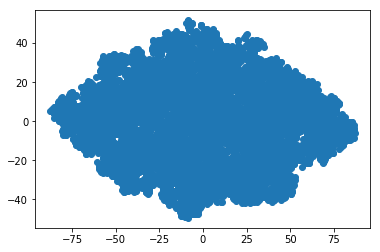
\includegraphics[width=3in]{Figures/ul0.png}
	\caption{t-SNE 2D Projection}
	\label{fig:tsne}
\end{figure}

\subsection{Initial Clustering}

\subsection{Clustering after symmetry transform}

\section{Conclusion}

\small{
\printbibliography
}

\end{document}
